%\section{Algorithm}\label{sec:optimization}



\subsection{Shape Refinement}\label{sec:refinement}

%there is still a need to refine the results that have not folded into pleasing results. 
Though not perfect, the initial 3D shape provides a good start point for generating the final carton model. 
%
To further refine the 3D shape, the 3D coordinates of all the vertexes are then refined based on a set of shape constraints, such as vertex merging, panel pasting, and so on.
%
%the main idea is to prescribe the shape constrains by a set of vertexes of the polymesh. 
%Moreover, with the extra information acquired from user interaction, we can finally construct the desired 3D realization.
In this step, the coordinate of vertexes are chosen as our objective instead of angles on folding edges, mainly because that the geometric constrains in 3D shapes can be more simply and intuitively represented by 3D vertex coordinates.
% and we can implement the algorithm introduced by Bouaziz et al. easily~\cite{Bouaziz:2012:SSD:2346796.2346802}.


%\subsection{Aided Detection}

%While the initial 3D model with simple angle folding provides a rough idea about the carton shape, 
A suggestive interface is provided to users for efficiently exploring better carton shapes, as described later in Sec.~\ref{sec:interaction}. 
%
Once the user selects a suggested shape refinement operation, we optimize the 3D shape based on a series of geometric constraints.
%We now introduce the constrains used in our construction method:
Given the current mesh whose vertex positions are defined as $\{\vo_i\}^{N}_{i=1}$, a new mesh with the same topology but new vertex positions $\{\vn_i\}^{N}_{i=1}$ will be computed according to the specified shape constraints.
%
The geometric constraints can be classified into two groups, shape rigidity constraints and shape modification constraints.
% 
First, to keep the rigidity of each panel, the constraints including panel rigidity and coplanarity, corresponding to the similarity constraint and plane constraints described in \cite{Bouaziz:2012:SSD:2346796.2346802}. 
%
Second, once vertexes or panels are confirmed to be merged to modify the rough shape, more constraints are added. 
%
Each constraint is defined as following.  

\comments{
\paragraph{Edge length constraint.} 
For each edge in $\{e_j\}_{j=1...M}$, its length should be preserved when refine the carton shape.
Hence, its two endpoints $\mathbf{v}_{js}$ and end point $\mathbf{v}_{jt}$ should satisfy 
\begin{equation}
||\mathbf{v}_{js} - \mathbf{v}_{jt}||^2 = ||\mathbf{\hat{v}}_{js} - \mathbf{\hat{v}}_{jt}||^2.
\label{equ:edge}
\end{equation}
%to ensure that the length of each edge stays the same.
}


\paragraph{Face rigidity} 
Each panel keeps its shape unchanged during folding. This constraint is defined by keeping the length of each line connecting any pair of points $\mathbf{v}_{a}, \mathbf{v}_{b}$ on the panel the same.
\begin{equation}
||\mathbf{v}_{a} - \mathbf{v}_{b}||^2 - ||\hat{\mathbf{v}}_{a} - \hat{\mathbf{v}}_{b}||^2 = \mathbf{0}.
\label{equ:plane}
\end{equation}




\paragraph{Coplanarity} {For each panel, the coplanarity constraint specifies that all vertexes in this panel should always lie on a plane. 
We can compute the sorted eigenvectors $\mathbf{U} = [\mathbf{e}_1, \mathbf{e}_2, \mathbf{e}_3]$ of the $ 3 \times 3$ covariance matrix $\mathbf{C}^T\mathbf{C}$ where $\mathbf{C} = \{\mathbf{v}_{kj}\}_{j=1}^{N_k}$, $\mathbf{v}_{kj}$ is the $j$th vertex among $N_k$ vertexes in the panel. By removing the last column of $\mathbf{U}$, we can implement plane projection as \cite{Bouaziz:2012:SSD:2346796.2346802} described.


If a set of shape modification operations, such as vertex merging and panel pasting, are selected, more constraints are added to optimizing vertex positions. 
%
%and one of the interaction is to choose the right given suggestion including points needed to be merged together. As for the point information, the constrains can be written like:

\begin{figure}
	\centering
	\subfigure[Vertex merging]{
		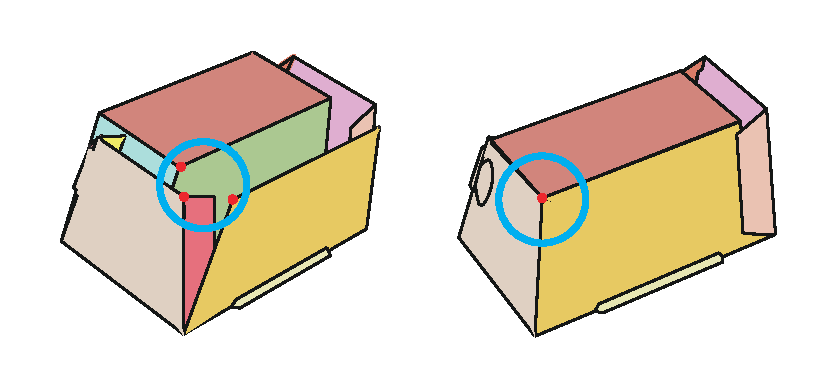
\includegraphics[width=0.45\columnwidth]{images/vertexmerging}
		\label{fig:vertexmergingBeforeAfter}
	}
	\subfigure[Panel pasting]{
		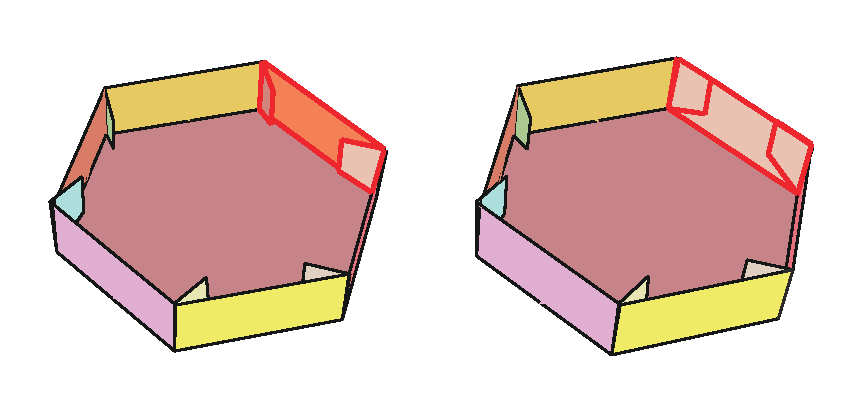
\includegraphics[width=0.45\columnwidth]{images/facemerging}
		\label{fig:facemergingBeforeAfter}
	}
	\caption{3D shape refinement based on merging vertexes (a), or pasting panels (b). The locations where the 3D shape changes are highlighted in blue.  }
	\label{fig:shaperefinement}
\end{figure}

\paragraph{Merging vertexes} 
For any two vertexes $\mathbf{v}_p$ and $\mathbf{v}_q$ that are selected to be merged as the same vertex, we have 
\begin{equation}
\mathbf{v}_p - \mathbf{v}_q = \mathbf{0}.
\label{equ:point}
\end{equation}
%if these two points $\mathbf{v}_p$, $\mathbf{v}_q$ need to be moved into the same place. 

\paragraph{Panel pasting}
%If a smaller face $f_a$ is snapped to a larger face $f_b$, for each vertex $\vn_i$ in the face $f_b$, we have
%\begin{equation} \label{eq:face-paste}
%\vn_i \cdot \mathbf{n}_a = 0,
%\end{equation}
%where $\mathbf{n}_a$ is the normal of the face $f_a$.
If two panels $P_a$ and $P_b$ need to snap together, the whole vertexes of these two panels should satisfy the coplanarity constrain. 


%When the above constrains still lead to an ill-posed problem, soft constraints will be added to keep the original positions of the vertices that are not relative to the shape modification. 

\reply{Typically only a few shape modificatiaon operations are selected at each time, the above constraints form an under-constrained system to solve the new vertex coordinates. In order to find feasible solution for the constrained problem,} soft constraints will be added to keep the original positions of the vertexes that are not relative to the shape modification.

\paragraph{Irrelevant vertexes} For the vertexes $\{\mathbf{v}_i\}$ are not in the same plane with any vertex for merging or panel pasting, they should stay at their original location. 
We add these soft constraints by adding a small weight $w$, which is set 0.001 in our experiments to the following equation. 
\begin{equation}
\mathbf{v}_i - \mathbf{\hat{v}}_i = \mathbf{0}.
\label{equ:irrelevant}
\end{equation}

\reply{\cite{Bouaziz:2012:SSD:2346796.2346802} proposed an efficient optimization method that could combines all these shape constraints together. We directly use their c++ library ShapeOp to solve our constraint optimization problem once a shape modification operation is performed.}
Figure~\ref{fig:shaperefinement} shows two examples of shape refinement by merging three vertexes and pasting three panels respectively. 

\comments{
Combining the above constraints, the new vertex locations can be solved by minimizing the proximity function based on projection operators~\cite{Bouaziz:2012:SSD:2346796.2346802}. 
%
\reply{For a single point $\mathbf{v}$, the proximity function is defined as
\begin{equation}
\phi(\mathbf{v}) = \sum_{i=1}^{m}\omega_i{d_i(\mathbf{v})}^{2},
\label{equ:function}
\end{equation}
where $\omega_i$ are non-negative weights, and $d_i$ is the distance between the point $\mathbf{v}$ and its projection onto the constraint set, $m$ is the number of constraints. For all the vertexes $\mathbf{V} = \{\mathbf{v}_i\}_{i=1\dots n}$, the shape proximity function is formulated as
\begin{equation}
\phi(\mathbf{V}) = \sum_{i=1}^{m}\omega_i||\mathbf{N}_i\mathbf{V}_i-P_i(\mathbf{N}_i\mathbf{V}_i)||_2^2,
\label{equ:function2}
\end{equation}
where $\omega_i$ are weights and $P_i(\cdot)$ is the projection onto the constraint. The matrix $\mathbf{N}_i$ is used to center the vertexes at their mean.
}
}
%

